\documentclass{beamer}
\usepackage{graphicx} 
\title{Domača naloga 1 pri predmetu NRO}
\author{Lan Enej Zirnstein}
\date{November 2024}

\begin{document}

\maketitle

\begin{frame}
    \frametitle{Kazalo}
    \tableofcontents[sectionstyle=show, subsectionstyle=show/shaded/hide]
\end{frame}

\section{Vsebina datoteke naloga1\_1.txt}
\begin{frame}{Vsebina datoteke naloga1\_1.txt}
    Datoteka \texttt{naloga1\_1.txt} vsebuje podatke, ki so strukturirani na naslednji način:
    \begin{itemize}
        \item Prva vrstica: parameter kateremu pripadajo podatki v spodnjih vrsticah
        \item Druga vrstica: število vrstic z vrednostjo t in število podatkov v vsaki vrstici
        \item Vsaka naslednja vrstica: posamezna vrednost časa t[s]
    \end{itemize}

    V primeru uporabe funkcije \texttt{importdata} so vhodni in izhodni podatki naslednji:
    \begin{itemize}
        \item \textbf{Vhodni podatki}: Ime datoteke, ki jo želite prebrati (v tem primeru \texttt{"naloga1\_1.txt"}), ter opcionalne nastavitve, kot so delimiterji (ločuje eno vrednost od druge) ali headerlines (število vrstic za preskočiti)
        \item \textbf{Izhodni podatki}: Funkcija \texttt{importdata} vrne matriko z vsebino datoteke. V tem primeru \texttt{importdata} vrne podatke iz datoteke, pri čemer so številčne vrednosti shranjene v matriki (ali vektorju)
    \end{itemize}
\end{frame}

\section{Graf funkcije P(t)}
\begin{frame}{Graf funkcije P(t)}
    Na podlagi prebranih podatkov smo ustvarili graf funkcije $P(t)$. Na x-osi prikazujemo čas ($t$) v sekundah, na y-osi pa moč ($P$) v vatih.
    \begin{figure}
    \centering
    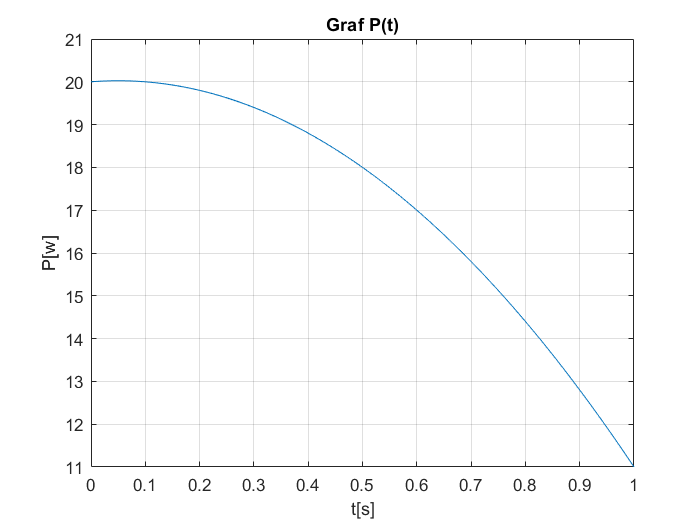
\includegraphics[width=0.7\linewidth]{slika grafa P(t).png}
    \caption{Graf 1: graf P(t)}
    \label{fig:enter-label}
    \end{figure}
\end{frame}

\section{Izračun integrala s trapezno metodo}
\begin{frame}{Izračun integrala s trapezno metodo}
    Trapezna formula za izračun integrala je podana kot:
    \[
    \int_{a}^{b} f(x) \, dx \approx \frac{\Delta x}{2} \left( f(x_0) + 2f(x_1) + 2f(x_2) + \dots + 2f(x_{n-1}) + f(x_n) \right)
    \]

    Rezultat integrala smo izračunali z MATLAB kodo, ki smo jo napisali ročno in s funkcijo \texttt{trapz}.

    \begin{itemize}
        \item \textbf{Rezultat z lastno kodo:} 17.1665
        \item \textbf{Rezultat z uporabo funkcije {trapz}:} 17.1665
    \end{itemize}
\end{frame}

\end{document}
